\sectiontinyvert{Code} \label{sec:code}
Our code, together with usage instructions, 
\ifanonymous{is given as part of the sup. mat. It can also be found in our anonymous project page\footnote{\label{footnote_github}\url{https://github.com/FLEX-2021/FLEX}.}
}
\else{is available on our project page\footnotemark[1]{}.}
\fi
The reader is encouraged to run the code and witness the reproducibility of our model.

\sectiontinyvert{Additional visualizations} \label{sec:media}

% 
\begin{figure*}[ptbh]
\centering
\setlength{\abovecaptionskip}{0pt plus 3pt minus 2pt}
\setlength{\belowcaptionskip}{-20pt plus 3pt minus 2pt}
\caption*{}
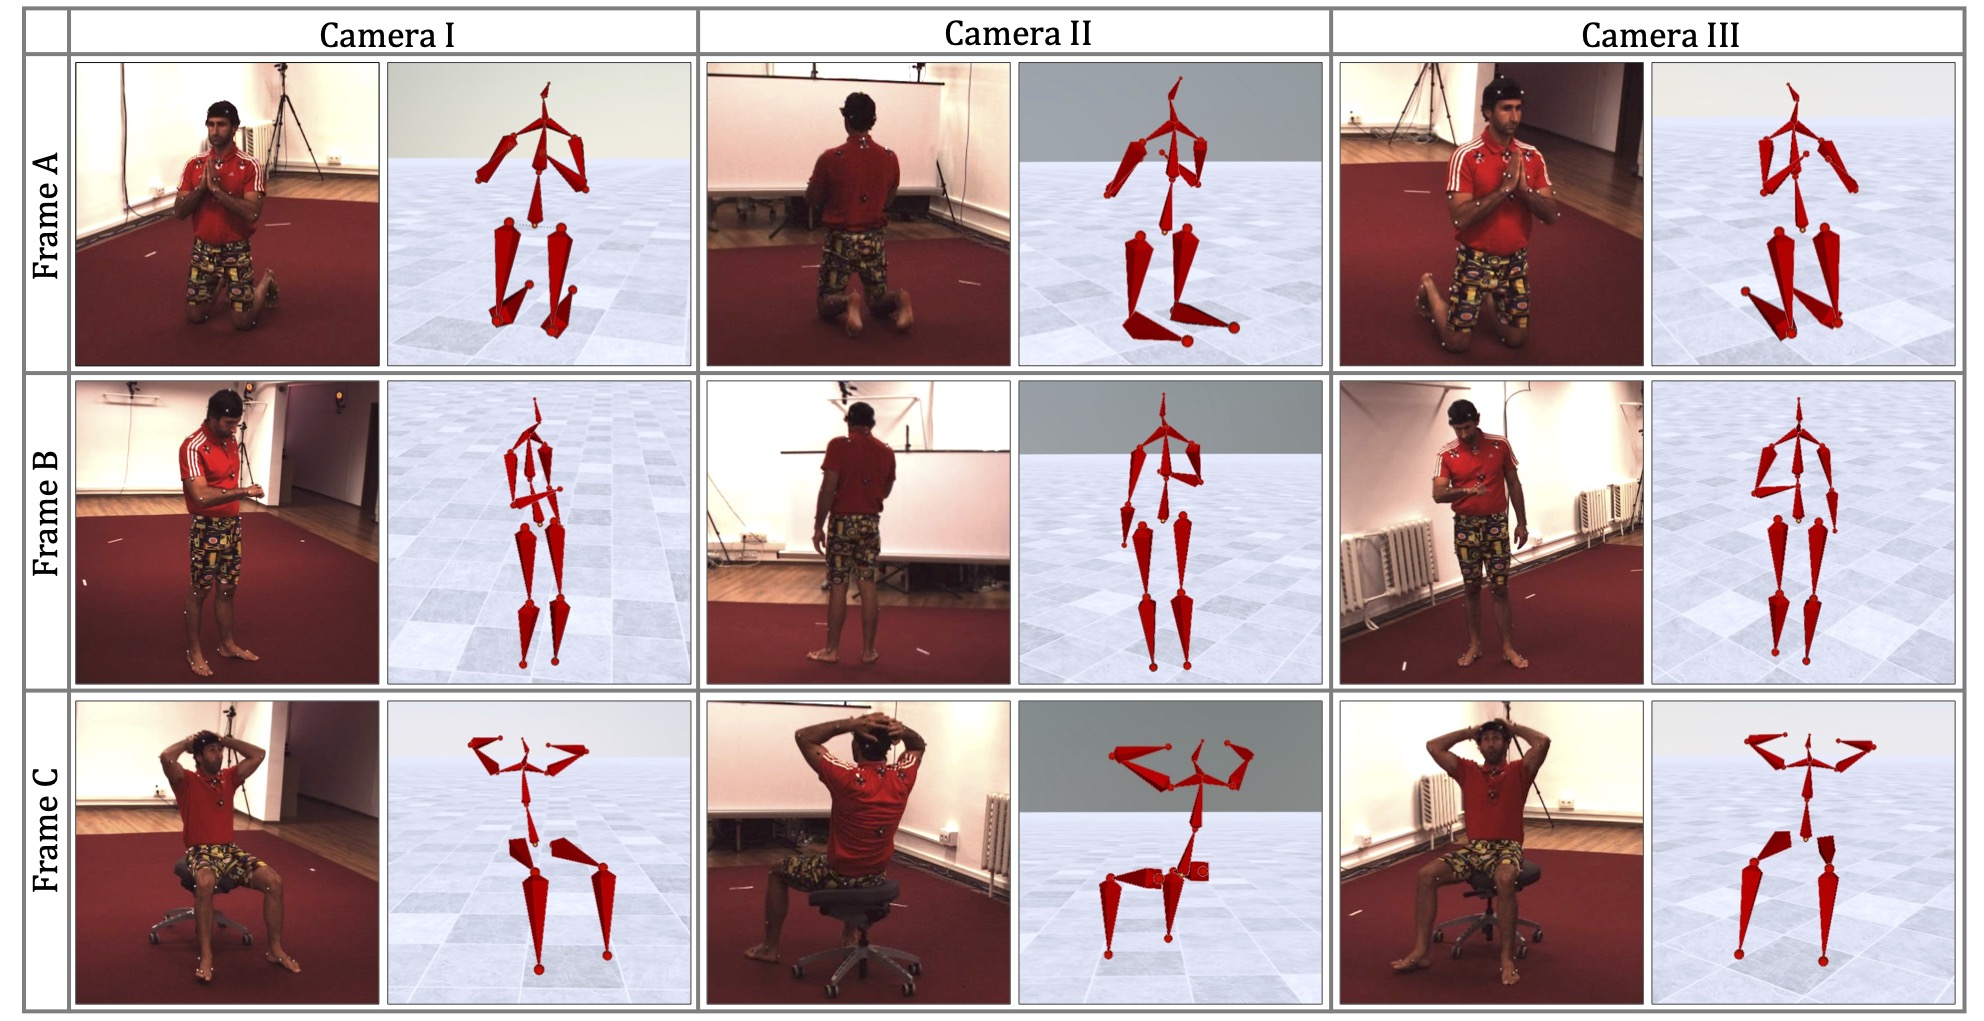
\includegraphics[width=.9\linewidth]{./images/H36M_results_second.jpg}
\setlength{\abovecaptionskip}{0pt plus 3pt minus 2pt}
\setlength{\belowcaptionskip}{0pt plus 3pt minus 2pt}
\caption{Additional results on videos from the Human3.6M dataset.}
\label{fig:quality_h36_b}
\end{figure*}

\begin{figure*}[ptbh]
\centering
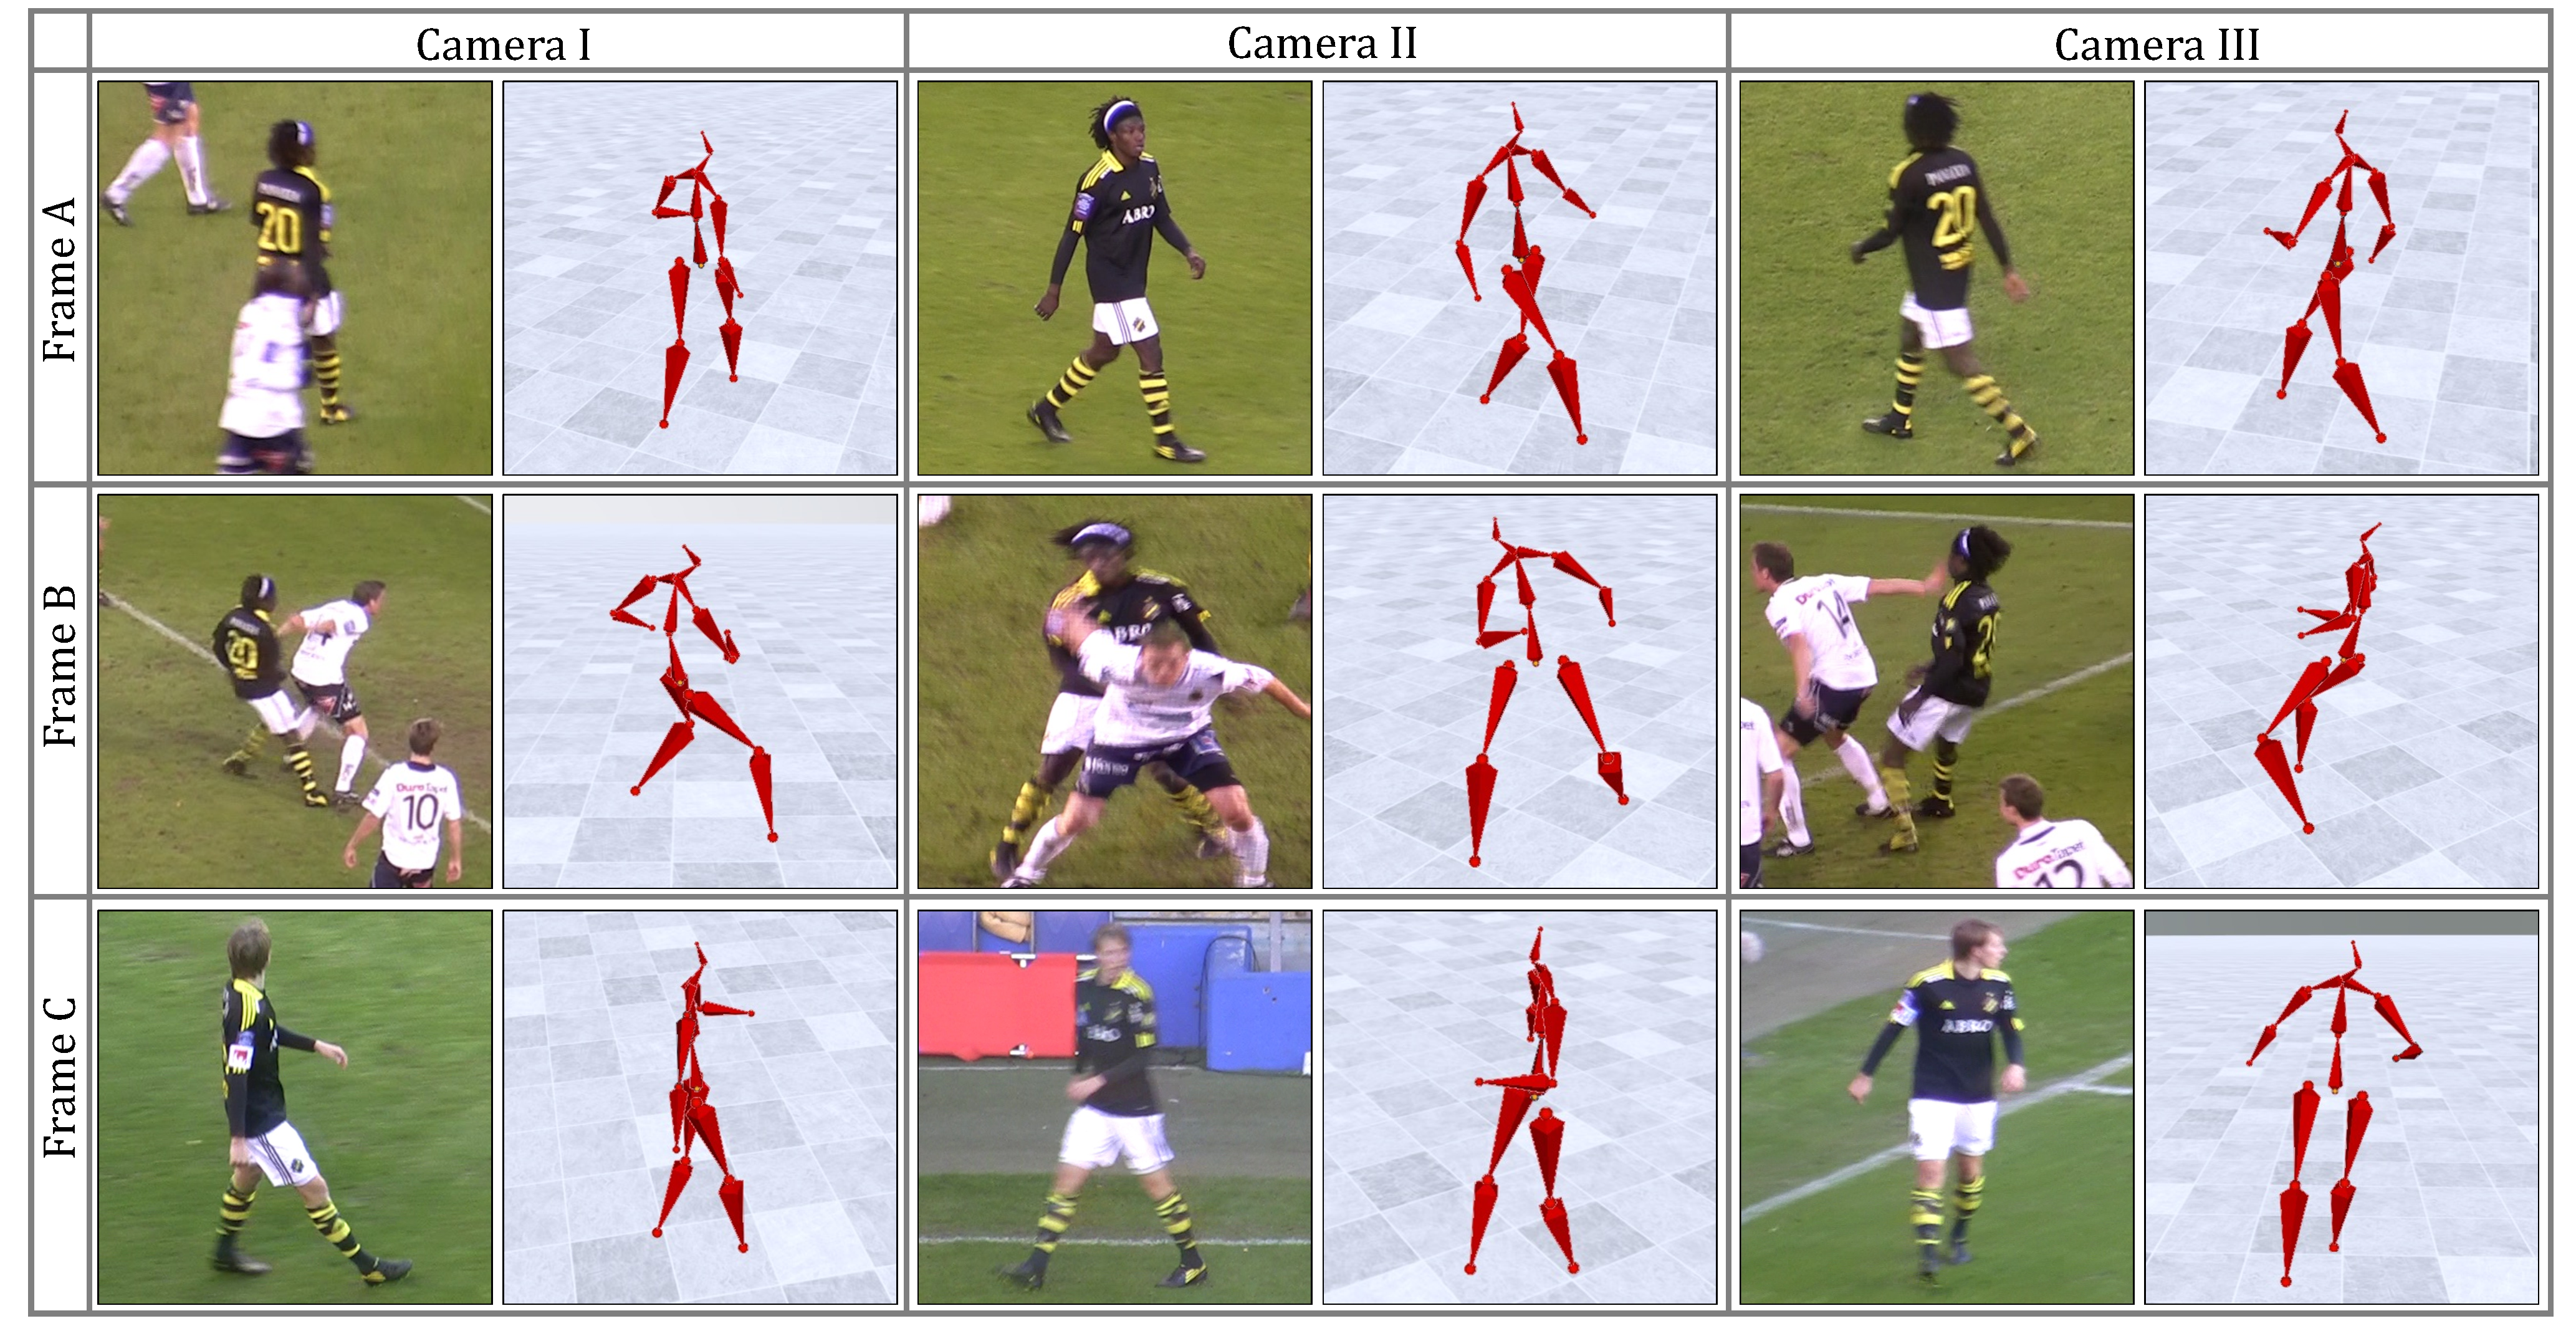
\includegraphics[width=.9\linewidth]{./images/Football_results_second.pdf}
\setlength{\abovecaptionskip}{3pt plus 3pt minus 2pt}
\setlength{\belowcaptionskip}{-7pt plus 3pt minus 2pt}
\caption{Additional results on videos from the KTH Multi-view Football II dataset. }
\label{fig:quality_KTH_b}
\end{figure*}

\begin{figure*}[tbh]
\centering
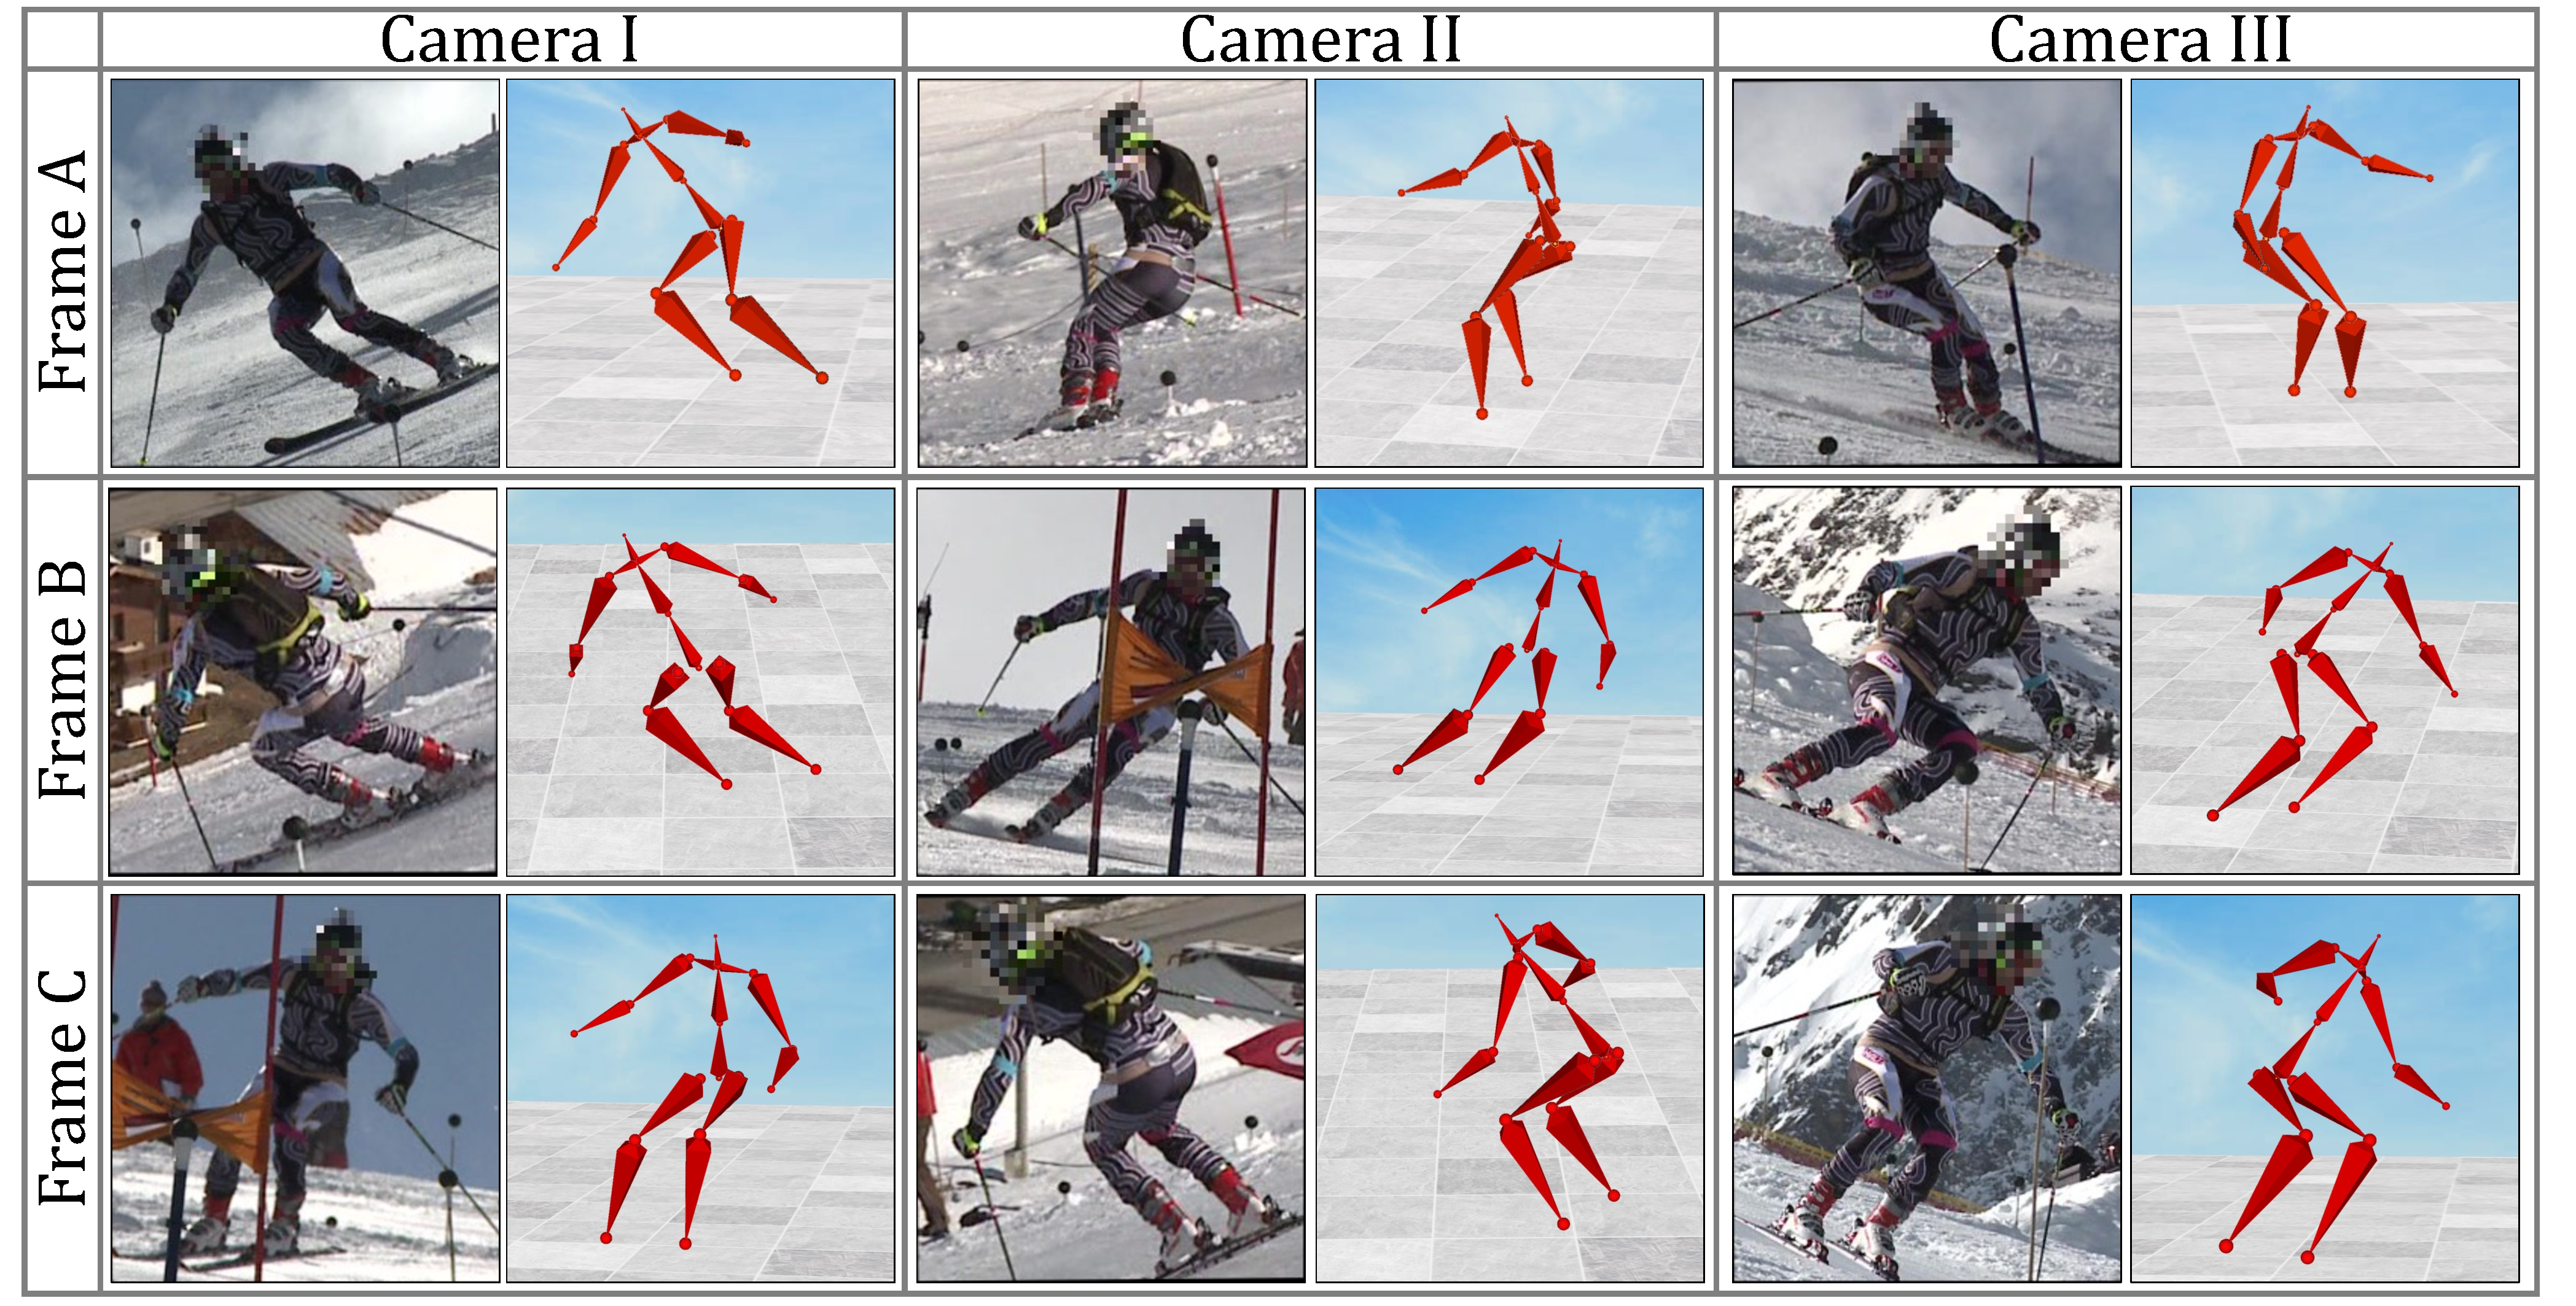
\includegraphics[width=.9\linewidth]{./images/Ski_results.pdf}
\setlength{\abovecaptionskip}{3pt plus 3pt minus 2pt}
\setlength{\belowcaptionskip}{-7pt plus 3pt minus 2pt}
% \caption{Results on the Ski-Pose PTZ-Camera dataset. Also shown (in small scale) in the main paper.  }
\caption{Enlarged results on the Ski-Pose PTZ-Camera dataset (from main paper).  }
\label{fig:quality_ski_large}
\end{figure*}

\begin{figure*}[tbh]
\centering
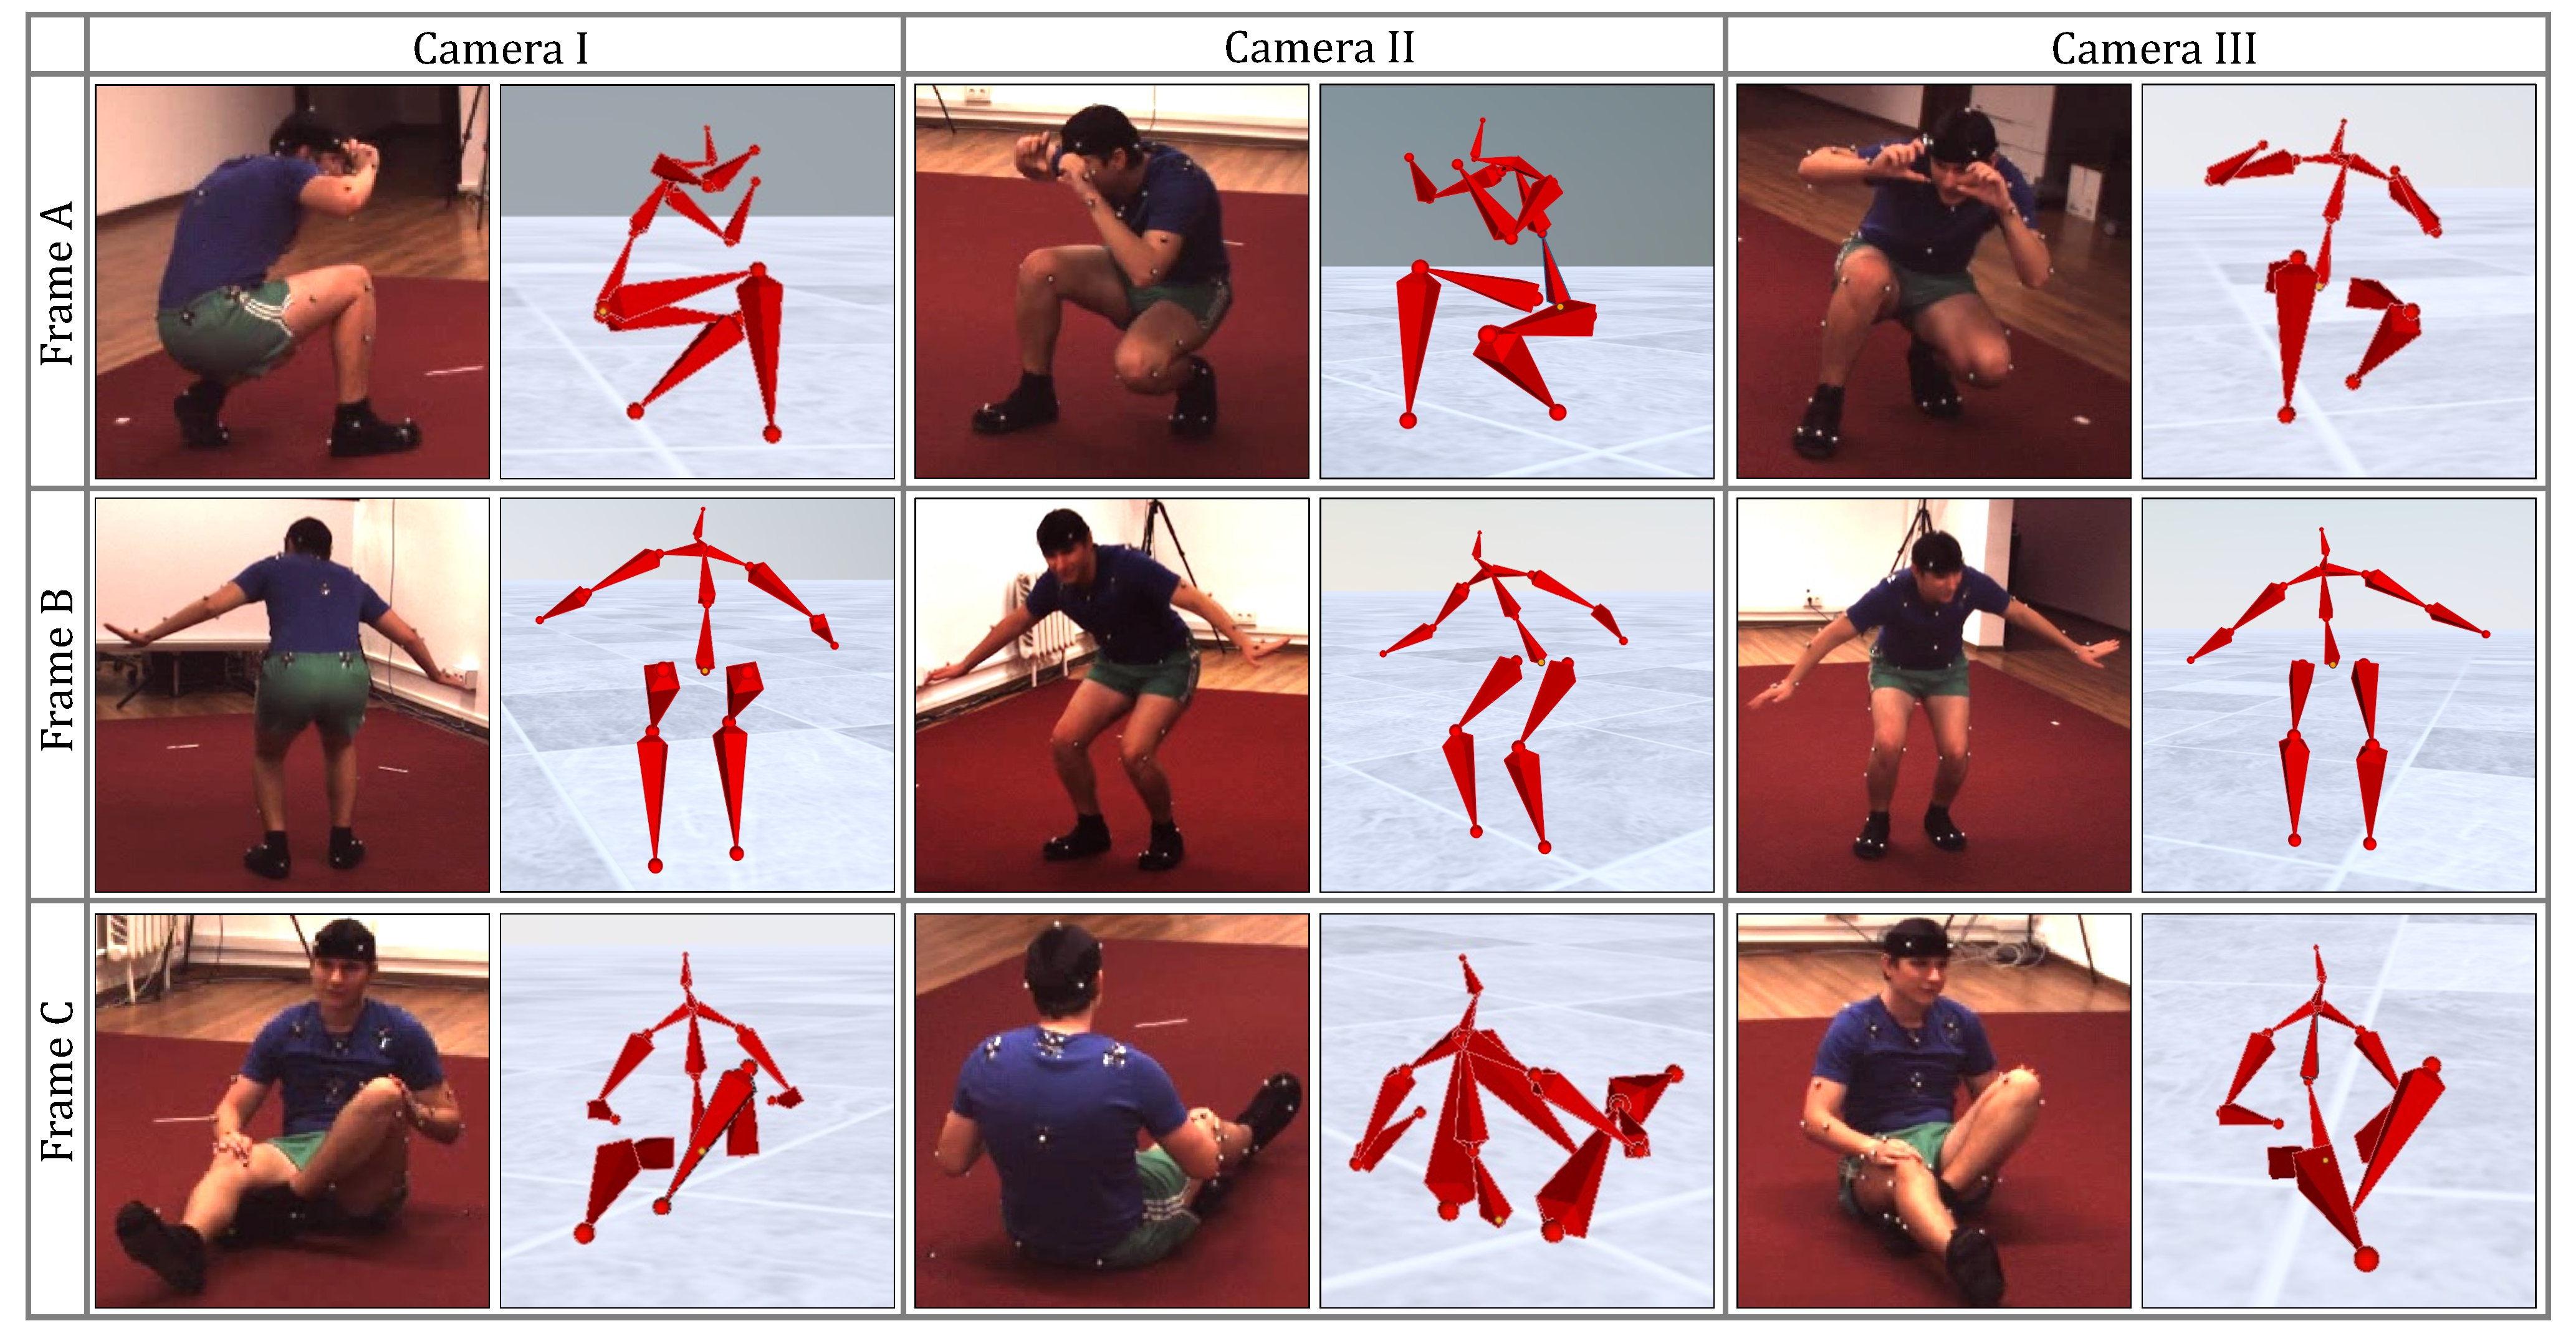
\includegraphics[width=.9\linewidth]{./images/H36M_results.pdf}
\setlength{\abovecaptionskip}{3pt plus 3pt minus 2pt}
\setlength{\belowcaptionskip}{-7pt plus 3pt minus 2pt}
\caption{Enlarged results on the Human3.6M dataset (from main paper).  }
\label{fig:quality_h36_large}
\end{figure*}

\begin{figure*}[tbh]
\centering
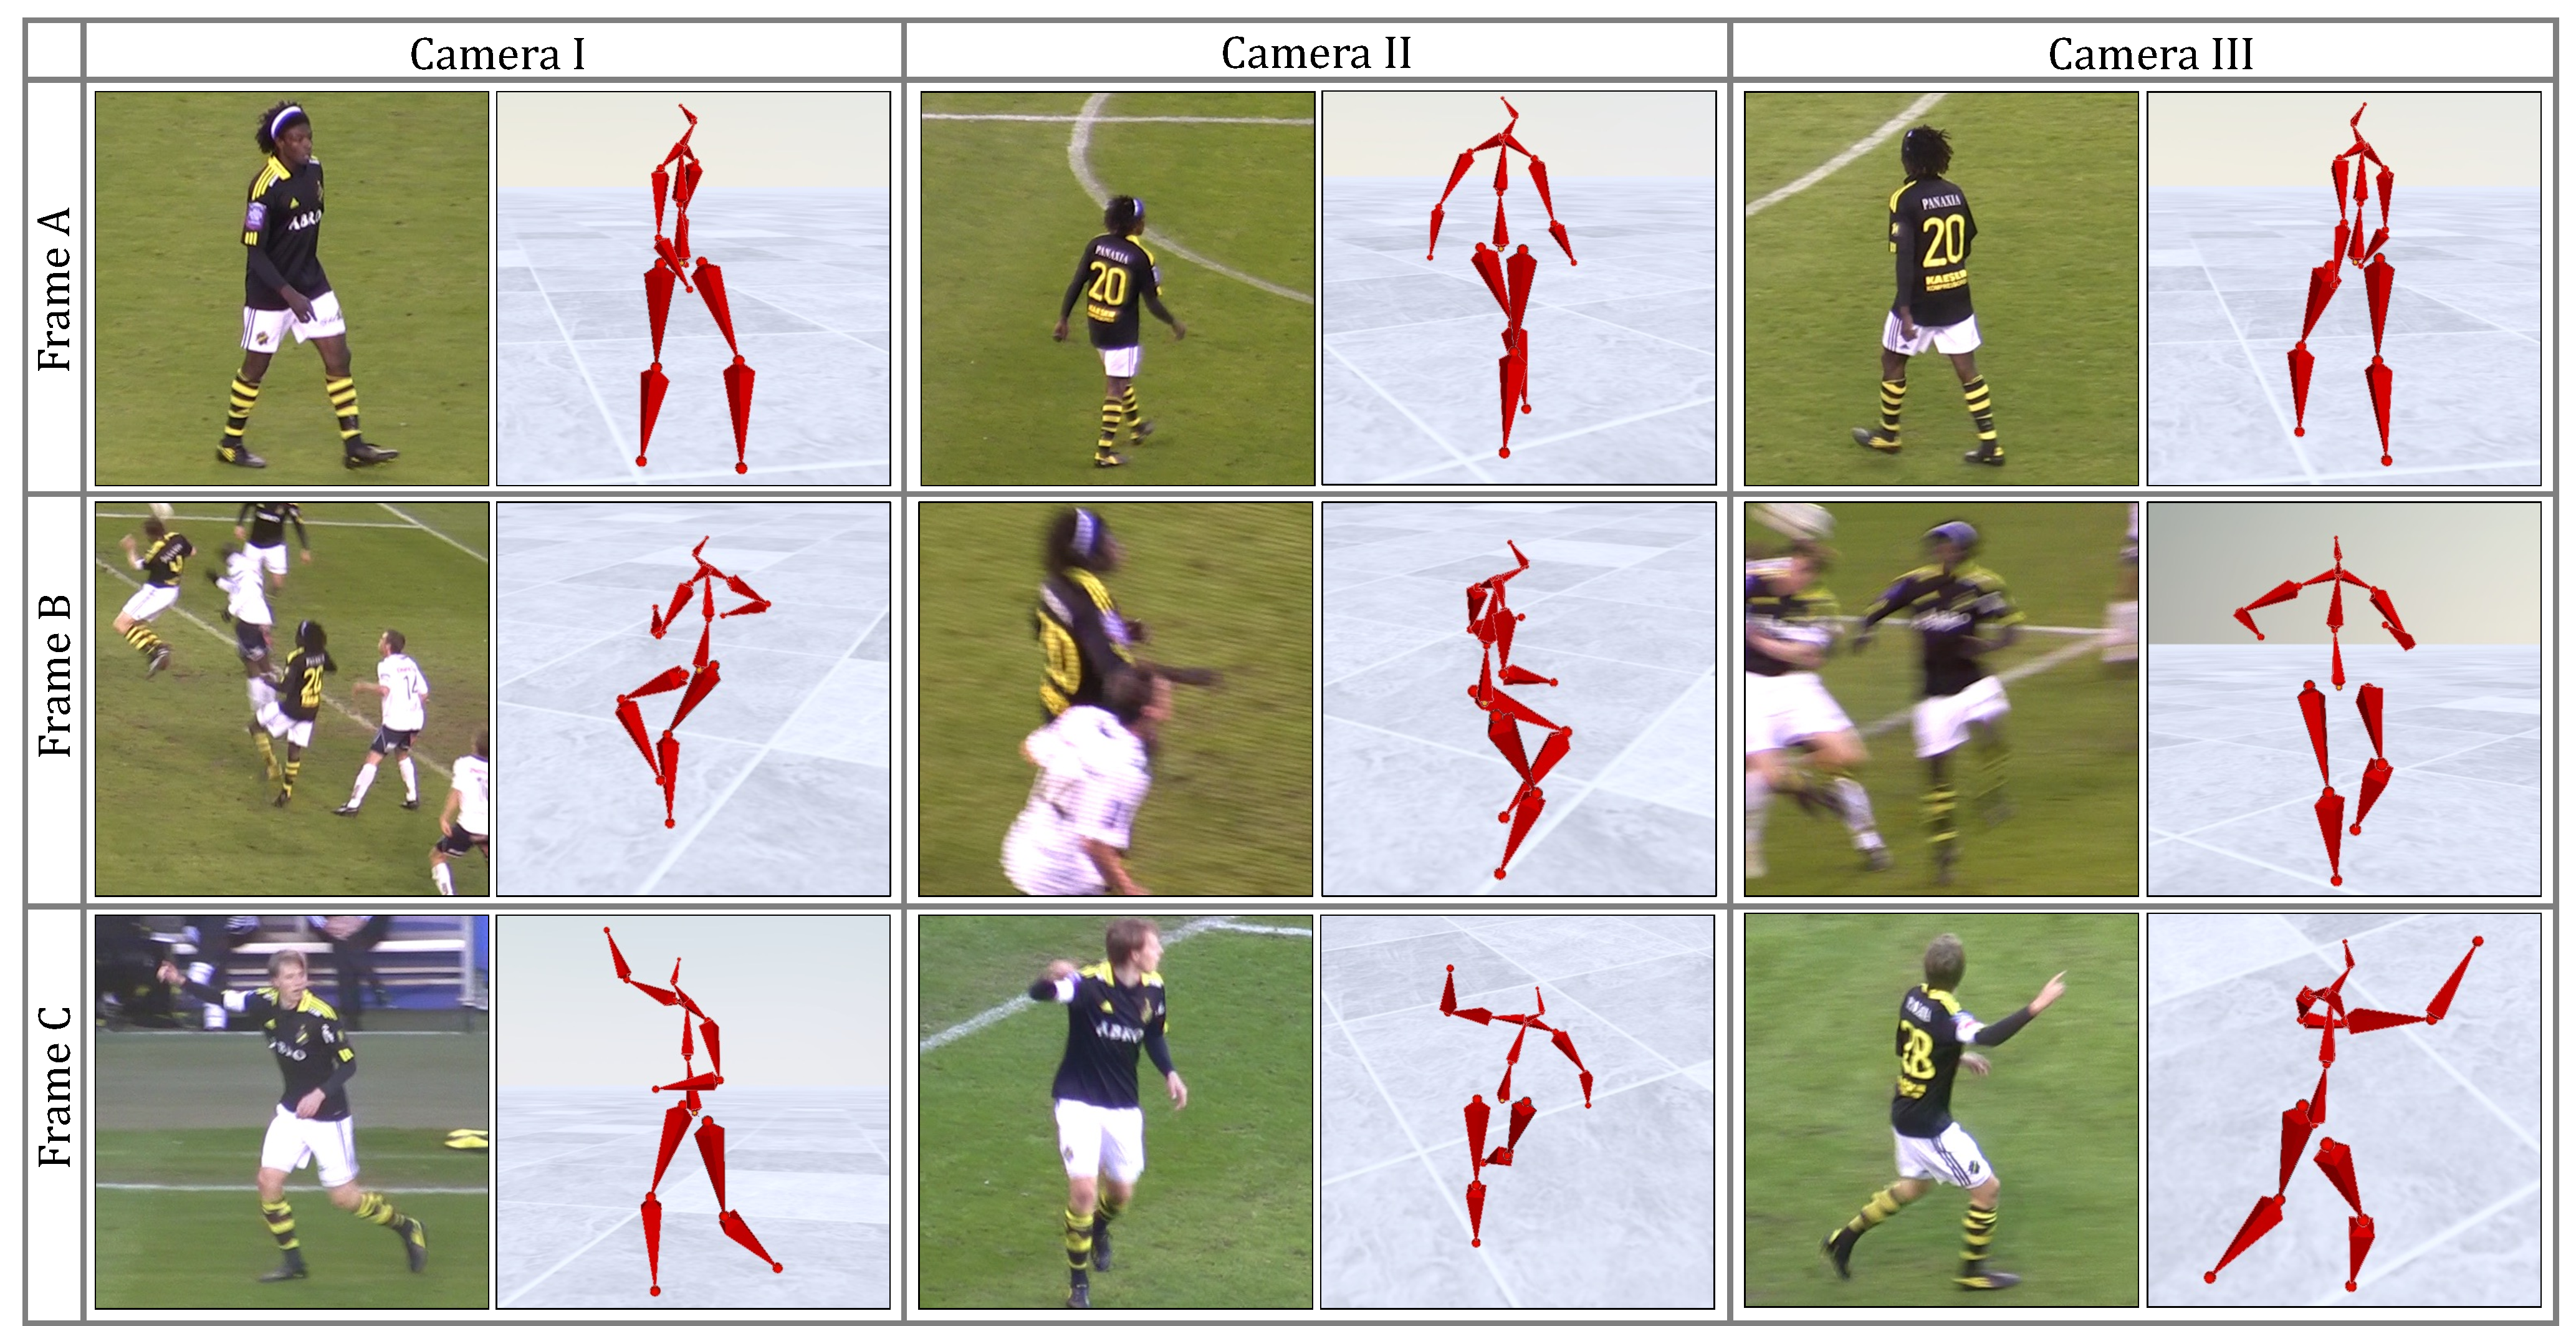
\includegraphics[width=.9\linewidth]{./images/Football_results.pdf}
\setlength{\abovecaptionskip}{3pt plus 3pt minus 2pt}
\setlength{\belowcaptionskip}{-7pt plus 3pt minus 2pt}
\caption{Enlarged results on the KTH Football II dataset (from main paper).}
\label{fig:quality_KTH_large}
\end{figure*}
 this file is inputted from sup_main_raw_text.tex

\ifanonymous{Together with this document, we provide supplementary video files.}
\else{On our project page\footnotemark[1], the reader can find attached video files.}
\fi % end ifanonymous
The reader is encouraged to browse the video files in full-screen size. 
\ifanonymous{
A higher quality version of these files can be found in our anonymous project page\footnotemark[1]. 
}
\fi% end ifanonymous
Here is their description:

\begin{itemize}
    \item A clip describing our work: clip.mp4
    \item Video files showing our results on the Human3.6M dataset: Human36M*.mp4
    \item Video files showing our results on the KTH multi-view Football II dataset: KTH\_football.mp4
    \item Video files comparing MotioNet (single-view) and Iskakov \etal~\cite{iskakov2019learnable} results versus ours: MotioNet\_comparison.mp4 and Iskakov\_comparison.mp4, respectively. 
\end{itemize}

Note that we present only results that use input obtained by 2D estimation (as opposed to ground truth). Thus, our input is affected by occlusion and blur. Yet, we are able to mitigate the noisy input by exploiting multi-view data, in an ep-free fashion.

\begin{figure}[tbh]
\centering
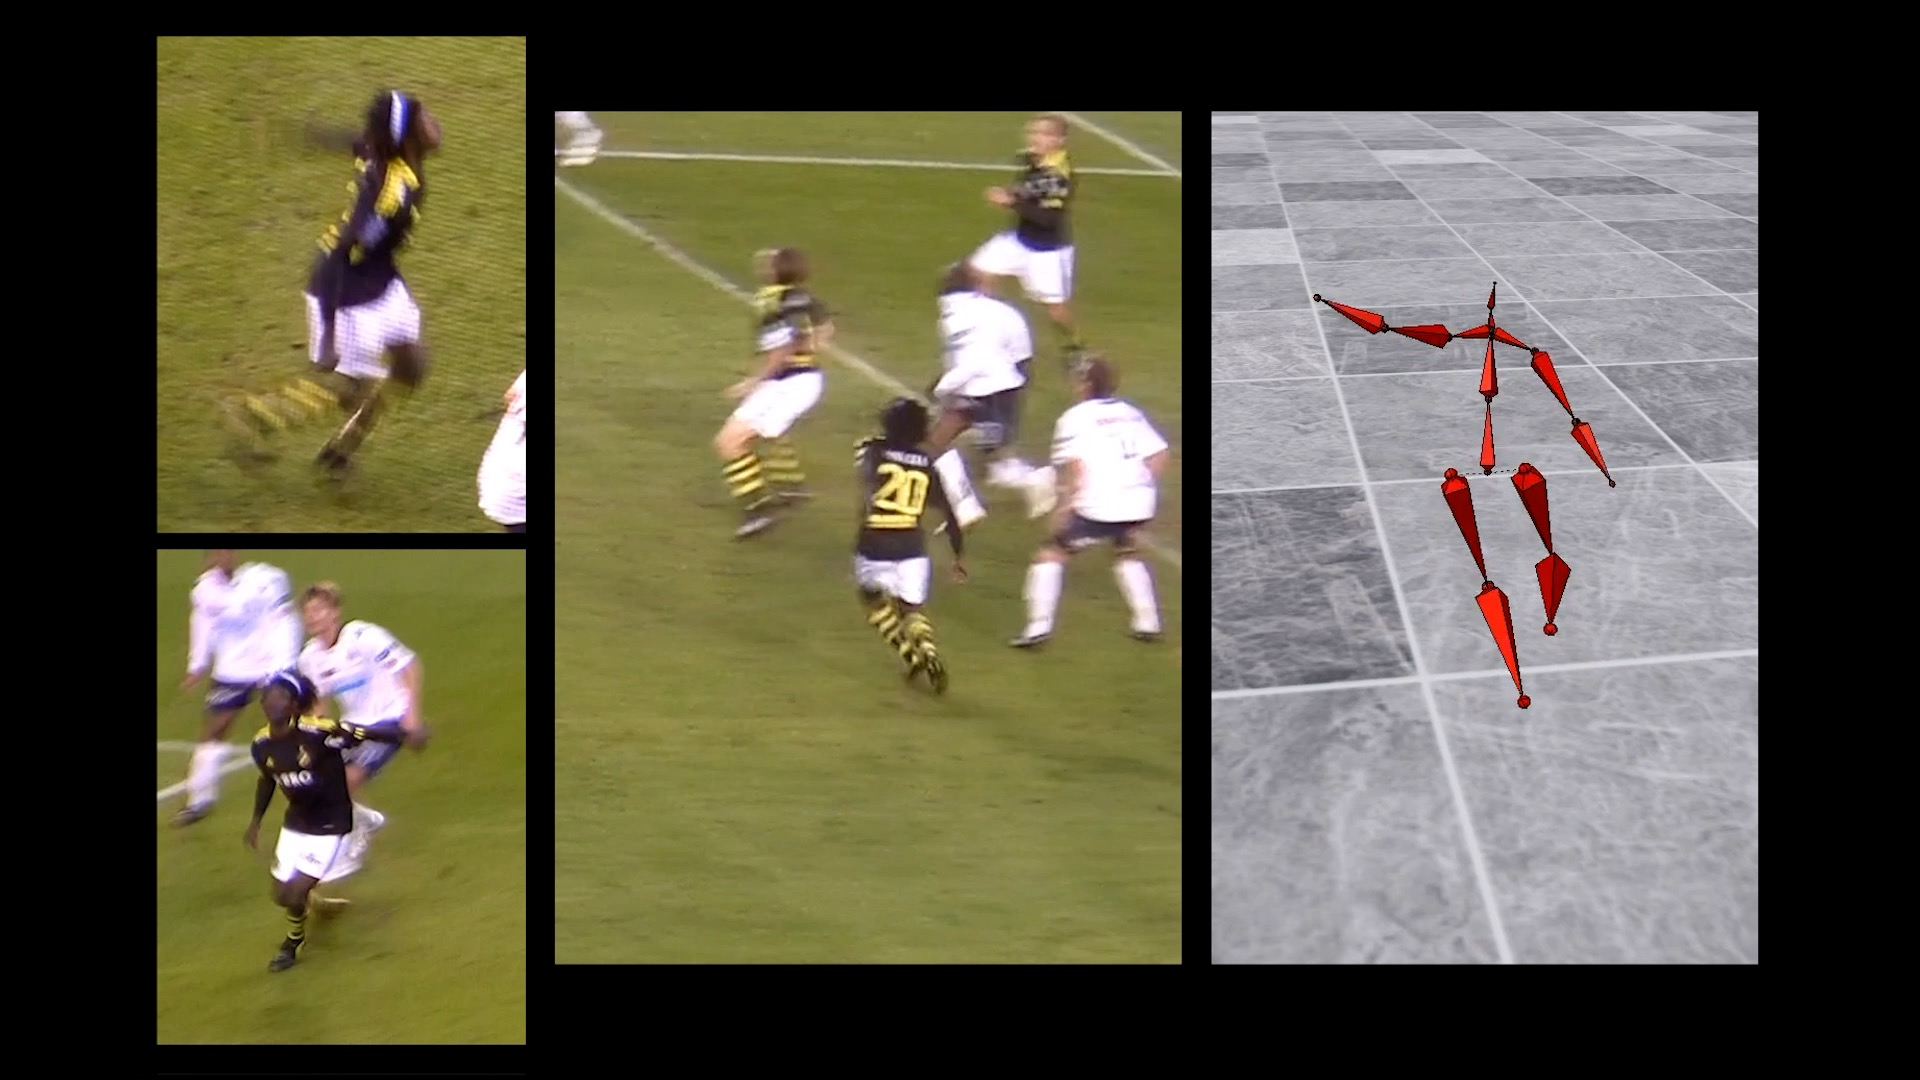
\includegraphics[width=\linewidth]{./images/football_hand_wave.jpg}
\setlength{\abovecaptionskip}{-5pt plus 3pt minus 2pt}
\setlength{\belowcaptionskip}{-5pt plus 3pt minus 2pt}
\caption{Our algorithm is able to grasp fine details. The player's left hand cannot be seen in the center view and is blurred in the left views. Yet, our model accurately reconstructs it. }
\label{fig:quality_football_hand_wave}
\end{figure}


In \Cref{fig:quality_football_hand_wave} we show how our algorithm is able to grasp fine details. The player's left hand cannot be seen in the center view and is blurred in the left views. Yet, our model accurately reconstructs it.

In \Cref{fig:quality_h36_b,fig:quality_KTH_b}, we show additional results on the Human3.6M and KTH Football multi-view II datasets. Each row depicts three views of one time frame. To the right of each image we place a reconstructed rig. 
%
\ifeccv{
\Cref{fig:quality_ski_large,fig:quality_h36_large,fig:quality_KTH_large} are enlarged versions of the figures shown in the main paper.
}\fi

\begin{figure}[tbh]
\centering
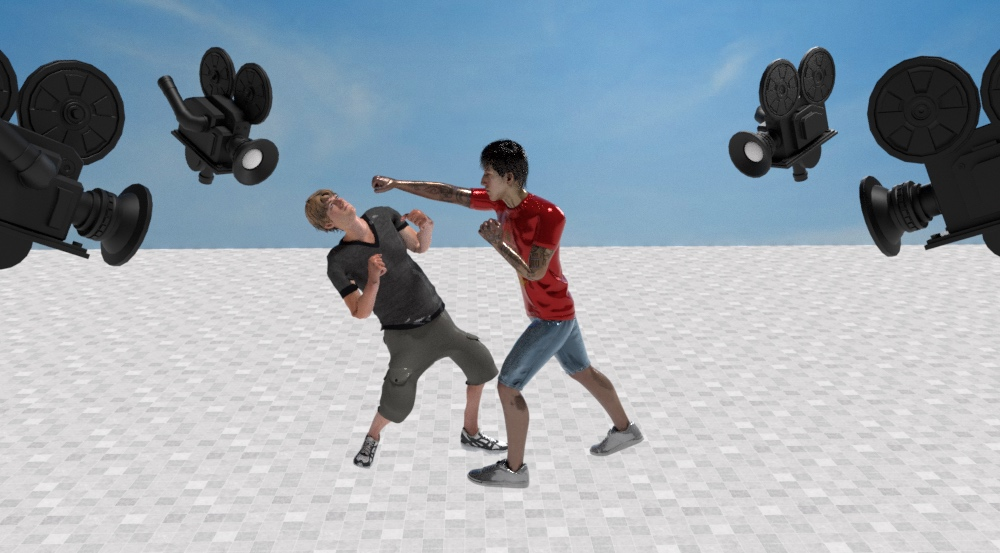
\includegraphics[width=\linewidth]{./images/Blender_studio.jpg}
\setlength{\abovecaptionskip}{-5pt plus 3pt minus 2pt}
\setlength{\belowcaptionskip}{-5pt plus 3pt minus 2pt}
\caption{Our "synthetic studio" created using Blender~\cite{blender} software with Mixamo~\cite{mixamo} 3D characters.
Two interacting characters are captured by multiple dynamic cameras and rendered into multiple video streams.}
\label{fig:blender_studio}
\end{figure}
\Cref{fig:blender_studio} shows our recording setup for creation of synthetic data. Note the depicted cameras, that dynamically move in the scene.

\begin{figure*}[tbh]
\centering
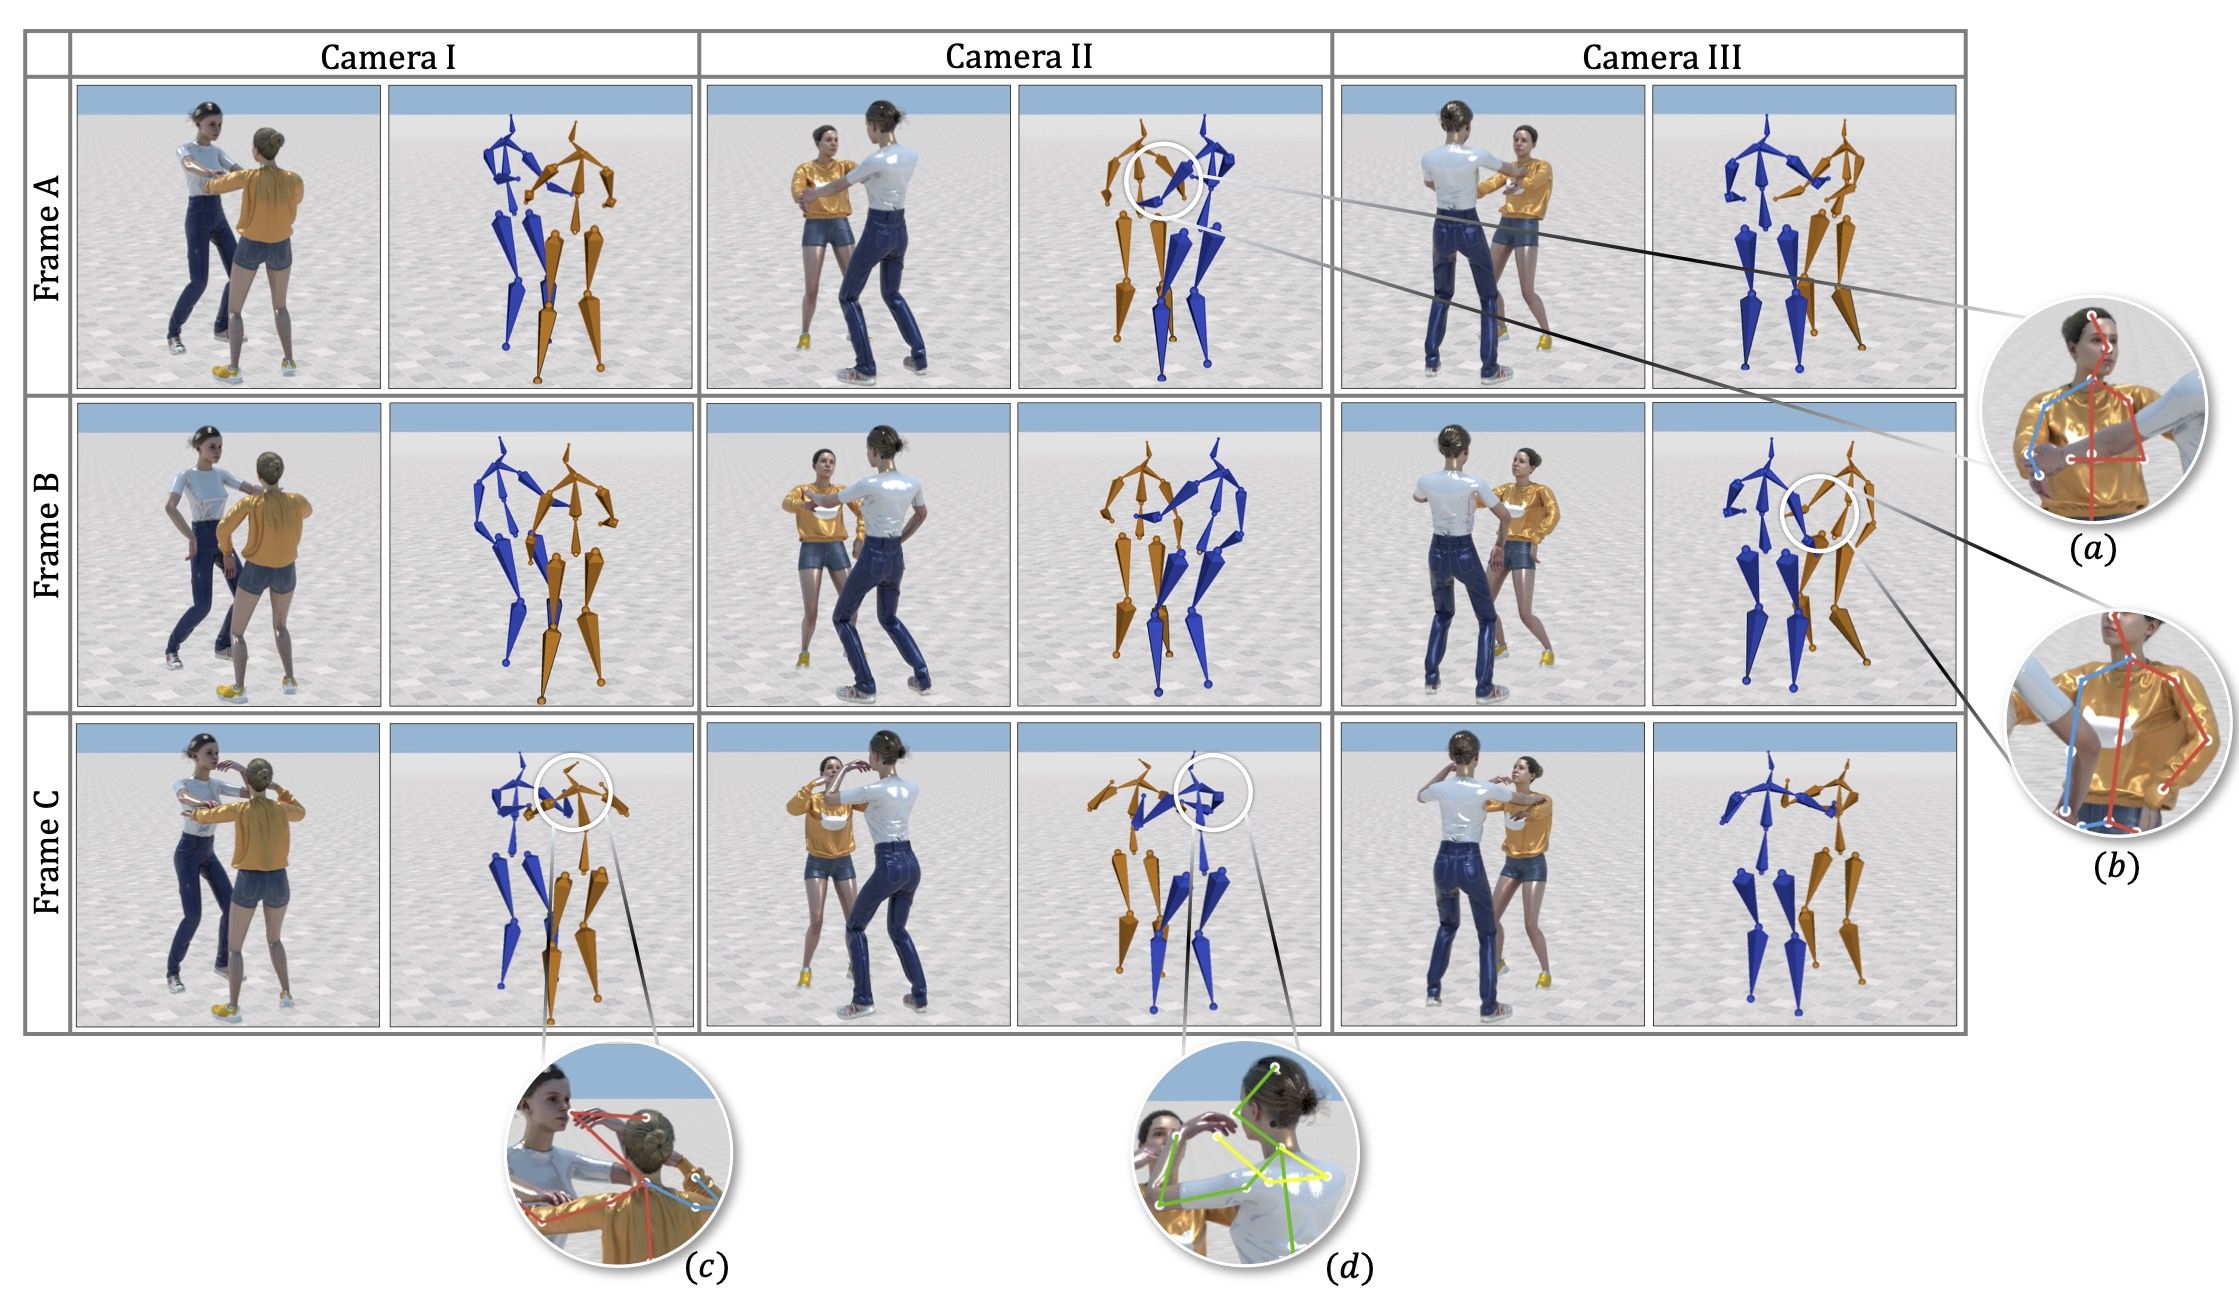
\includegraphics[width=\linewidth]{./images/Macarena_results_with_circles.jpg}
\setlength{\abovecaptionskip}{-10pt plus 3pt minus 2pt}
\setlength{\belowcaptionskip}{-10pt plus 3pt minus 2pt}
\caption{Our results on multi-person synthetic videos, picturing two Macarena dancers. Some of the 2D joints, used as input to our method, are severely inaccurate. However, our method is able to reconstruct correct 3D motion. In the following examples, let \emph{white dancer} and \emph{orange dancer} denote the dancer wearing a white and an orange shirt respectively. Several 2D based skeleton error examples are depicted in the zoomed-in circular insets: 
(a) Wrong pose estimation of the left arm of the orange dancer;
(b) The right arm of the orange dancer is occluded hence detected erroneously; 
(c) The nose tip of the orange dancer is erroneously detected as the nose tip of the white dancer;
(d) Erroneous 2D pose estimation of the white dancer's right hand.}
\label{fig:macarena_results_with_circles}
\end{figure*}
In \Cref{fig:macarena_results_with_circles} we depict qualitative results for a scene with two macarena dancers. We emphasize several viewpoints where the 2D backbone attains large errors. Yet, FLEX is able to compensate for these errors by fusing multi-view information.
\Cref{fig:fight_2d,fig:macarena_2d} depict 2D joint locations estimated by the AlphaPose~\cite{alphapose} backbone. A close look at these figures shows that many of the estimated locations are inaccurate, e.g., a hand of one subject is confused with the hand of the other subject. Even though the number of 2D errors is large, our algorithm is able to reconstruct the characters correctly.

